%% pdflatex BS_Report.tex && open BS_Report.pdf

\documentclass[11pt,margin=1in]{article}
\usepackage[margin=1in]{geometry}         % Document setup
\usepackage{graphicx}                     % Including pictures
\usepackage{amsmath}                      % Math mode
\usepackage{amssymb}                      % Math mode symbols
\usepackage{tikz}                         % For drawing example boxes
\usepackage{algorithm2e}                  % For including box mesh algorithm
\usetikzlibrary{shapes}                   % For the 'circle' shape
\renewcommand{\familydefault}{\sfdefault} % Setting the font


\begin{document}

\begin{center}
  \textbf{Box Spline Mesh Algorithm Summary}\\
  June $\text{5}^\text{th}$, 2017\\
  Thomas Lux
\end{center}


Given data $N = \{x_1, x_2, \dots, x_n\}\ |\  x_i \in \mathbb{R}^d$, and
associated response values $\{y_1, y_2, \dots, y_n \}$.

\section{Construct Box Mesh}
Each box in the box mesh will be specified by a center $c \in \mathbb{R}^d$,
lower width $l \in \mathbb{R}^d$, and upper width $u \in \mathbb{R}^d$. 
A point $x_i$ is contained by a box if $(1 \leq j \leq d) (c_j - l_j < x_{i,j} < c_j + u_j)$.
A two dimensional visual example of the containment region of a box, as we refer to it:

\vspace{1mm}

\begin{center}
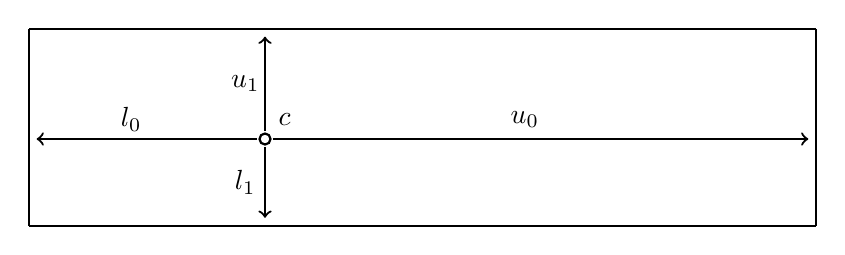
\begin{tikzpicture}[scale=1]

  \draw[thick] (3,1.1) circle (0.7mm);

  %% Draw arrows for each width
  \draw[thick,->] (3,1.2) -- (3,2.4);
  \draw[thick,->] (3,1.0) -- (3,0.1);
  \draw[thick,->] (3.1,1.1) -- (9.9,1.1);
  \draw[thick,->] (2.9,1.1) -- (0.1,1.1);

  %% Draw boundary of box
  \draw[thick,-] (0,0) -- (10,0);
  \draw[thick,-] (10,0) -- (10,2.5);
  \draw[thick,-] (10,2.5) -- (0,2.5);
  \draw[thick,-] (0,2.5) -- (0,0);

  %% Add text to the picture
  \node at (3.25,1.35) {$c$};
  \node at (1.3,1.35) {$l_0$};
  \node at (6.3,1.35) {$u_0$};
  \node at (2.75,0.55) {$l_1$};
  \node at (2.75,1.8) {$u_1$};

\end{tikzpicture}
\end{center}

The only restriction is that all widths must be greater than
zero. This means that $\text{min}_i\ l_i > 0 $ and $\text{min}_i\ u_i
> 0$. First, order the data in $N$ appropriately (discussed later),
initialize a single box with $c = x_1$ and lower and upper widths of
infinity.  Now, proceed to add the rest of the points in $N$ by:

\vspace{3mm}

\begin{algorithm}[H]
 \For{$i = 2, \cdots, n$}{
  Identify boxes $\mathbf{B}$ that contain $x_i$\;
  Initialize box \textit{m} with center $x_i$ that contains all boxes in $\mathbf{B}$\;
  \For{$b$ in $\mathbf{B}$}{
    split dimension := $\text{max}_j$ $|\text{b-center}_{j}-\text{m-center}_{j}|$\;
    Adjust the widths of $b$ and \textit{m} in \textit{split dimension}\\
    to be the difference between the centers in that dimension.
  }
 }
\end{algorithm}

\section{Evaluating A Box}
Interpolating and approximating requires using a set of boxes as
regions of influence for response values. Given a new data point $x$
is contained by a box $b$ (with associated $c$,$l$,and $u$), we
evaluate $b(x)$ as:

\begin{enumerate}
\item Scale $x$ according to the lower and upper widths of $b$ such
  that all $x_j < c_j$ map to $(0,0.5)$ and all $x_j > c_j$ map to
  $(0.5,1)$.
\item Scale this box-normalized $x$ to be in the appropriate range for
  the order of B-Spline chosen ($\times 2$ for order 2,$\times 3$ for order 3, etc.)
\item Take the product of the B-Splines along each dimension for the
  box spline normalized $x$ value. $\prod_{j=1}^{d} f(x_j)$ where $f$
  is the piecewise polynomial defining the b-spline of the desired order.

\end{enumerate}

\section{Interpolate $y$ for new $x$}

Identify the set of boxes $\mathbf{B} = \{b_i\ |\ b_i\ \text{contains}\ x\}$.
Calculate the estimated response value by
$$\frac{\sum_{b\in\mathbf{B}}b\text{-response} \times b(x)}{\sum_{b\in\mathbf{B}}b(x)}$$
where $b\text{-response}$ is the response value associated with each
box. Notice that this is using the box functions as a weighted sum.

\section*{Notes}

The ordering that has been used when adding points to the box mesh thus far is:

\begin{itemize}
\item Add the $x_i$ with the median valued $y_i$.
\item Compute the approximation surface error at all remaining $x_i$,
  add the $x_i$ to the surface with the most (relative) error.
\item Repeat previous step until small enough maximum error is obtained.
\end{itemize}

It is important to note that this constant recalculation of error
causes an increase in the runtime by a factor of $n$.

\end{document}


%===============================
%     Old Report (too long)     
%===============================

\begin{table}[!htbp]
\centering
\begin{tabular}{cc}

  Linear Box Mesh Interpolation & Quadratic Box Mesh Interpolation \\
  \vspace{1mm} & \\

  \includegraphics[width=7cm]{Linear_Box_Mesh} &
  \includegraphics[width=7cm]{Quadratic_Box_Mesh} 

\end{tabular}
\end{table}

\vspace{-10mm}

\section{Introduction}

This documents contains a brief explanation and analysis of the
\textit{Box Mesh} algorithm for generating an interpolating and/or
approximating surface to data given a desired error tolerance and
smoothness. The box mesh algorithm attempts to generate the smallest
set of overlapping boxes with the largest minimum side length (least
skinny) such that each box contains only one data point and the error
at all data points is below a given tolerance. After constructing this
set of boxes, we can use a variety of different functions to generate
the weight of a control point within each individual box. Taking a
weighted sum of control point values using these box functions
generates the surfaces seen above.

First we discuss the specification of each individual box and analyze
the use of linear and quadratic Box Splines as the box functions.
Then, we outline the box mesh construction algorithm, providing a
visual example. Following the example we discuss some mechanisms for
smoothing the surface. Finally, we conclude with a runtime analysis of
the box mesh algorithm.

\section{Box Specification}

A box mesh is composed of individual boxes. Each n-dimensional box has
a \textit{center} (c), \textit{lower width} (l), and \textit{upper
  width} (u). Given we are working in $d$ dimensions, a point $p$ is
inside of a box $b$ with center $c$, lower width $l$, and upper width
$u$ if $(\forall$ $i$ $|$ $0 \leq i < d)(c_i-l_i < p_i < c_i+u_i)$.
See the following visualized example of a box in 2 dimensions.


\subsubsection*{Box Functions}

Allowing for the conditional scaling of points, we can assume that
every box is a unit cube with center $(\frac{1}{2},\frac{1}{2})$. All
of our box functions then only need to be defined on the unit cube in
$d$ dimensions. The two functions that we utilize are: the linear box
spline defined by the direction vector set $[ I I ]$ where $I$ is the
d-dimensional identity matrix; and the quadratic box spline defined by
the direction vector set $[ I I I ]$. The convenience of restricting
ourselves to box splines of this form is that the box spline value at
any $x$ is simply the multaplicative sum $\Pi_{i=0}^{d-1} f(x_i)$
where $f$ is the piecewise polynomial that defines the associated
linear or quadratic B-Spline in one dimension.

We chose these two box functions because the linear box spline is
$c_0$ and the quadratic box spline is $c_1$. When normalizing any
arbitrary box into the unit cube with center
$(\frac{1}{2},\frac{1}{2})$ it is necessary that values be scaled
differently depending on which side of the center they are on. It is
clear that scaling the $x$ has no effect on the function value (we
maintain $c_0$), and since the first derivative of any box spline at
the center coordinate is 0 we do not break $c_1$ continuity with this
non-uniform scaling. But, the continuity of any derivative that is
non-zero at the center would lost with higher order box splines.

The output of the box functions will be used as the weight for the
control point value at the center of each box. Thus, the response
value associated with a given $x$ is computed by taking:

$$ \frac{\sum_{i=0}^{\mathbf{b}-1} \mathbf{b}_i(x) \cdot \text{boxval}_i}{\sum_{i=0}^{\mathbf{b}} \mathbf{b}_i(x) } $$

where $\mathbf{b}$ is the set of boxes that contain $x$,
$\mathbf{b}_i(x)$ is the value of the $i^{\text{th}}$ box function
evaluated at $x$, and $\text{boxval}_i$ is the response value
associated with the $i^{\text{th}}$ box.

\begin{table}[!htbp]
\centering
\begin{tabular}{cc}
  Linear Box Splines in 1 and 2 Dimensions & Quadratic Box Splines in 1 and 2 Dimensions \\

  \vspace{1mm} & \\

  \includegraphics[width=7cm]{Linear_1D} & \includegraphics[width=7cm]{Quadratic_1D} \\
  \includegraphics[width=7cm]{Linear_2D} & \includegraphics[width=7cm]{Quadratic_2D}   

\end{tabular}
\end{table}

\section{Box Mesh Construction}

Given a data set with $N$ points in $D$ dimensions, we want to
construct a set of $B$ boxes centered about $B$ points from the data,
referred to as control points. In order to create good response
approximations, we want to ensure that the boxes are both reasonably
shaped (not extremely skinny) and maximally overlapping. The box mesh
construction algorithm creates a set of boxes that each meet these two
criteria as well as contain strictly \textit{one} control point. This
final extra condition allows for strict interpolation.

The algorithm for the box mesh construction proceeds as follows:

\vspace{3mm}

\begin{algorithm}[H]
 \KwData{N by D+1 matrix of data where the last dimension is the response.}
 \KwResult{B-box mesh}
 Initialize one box with upper and lower widths of infinity at median response point\;
 \While{max error $>$ tolerance}{
  Identify point $p$ with max error\;
  Identify boxes $\mathbf{b}$ that contain $p$\;
  Initialize box \textit{new} with center $p$ that contains all boxes in $\mathbf{b}$\;
  \For{$b$ in $\mathbf{b}$}{
    split dimension := $\text{max}_i$ $|\text{b-center}_{i}-\text{\textit{new}-center}_{i}|$\;
    Adjust the widths of $b$ and \textit{new} in \textit{split dimension}\\
    such that $b$ and \textit{new} do not contain each other's center\;
  }
 }
 \caption{Box Mesh Construction}
\end{algorithm}

\vspace{10mm}

\subsubsection*{Visual Example of Box Mesh Construction}

The following 3 examples are all for x with dimension 2. The initial
boxes seen on the left are the $\mathbf{b}$. These boxes contain the
new point that will be added. The premise is that the new point has
already been identified as the one with the most error in
response. The resulting boxes seen on the right demonstrate the
reshaping of the new and old boxes.

\begin{table}[!htbp]
  \centering
  \begin{tabular}{cc}
    \includegraphics[width=7.5cm]{1-Before} & \includegraphics[width=7.5cm]{1-After} \\
  \end{tabular}
  \caption{Adding the blue point, reshaping the x-dimension of the orange box.}
\end{table}

\begin{table}[!htbp]
  \centering
  \begin{tabular}{cc}
    \includegraphics[width=7.5cm]{2-Before} & \includegraphics[width=7.5cm]{2-After} \\
  \end{tabular}
  \caption{Adding the orange point, reshaping the y-dimension of the
    blue and green boxes.}
\end{table}

\begin{table}[!htbp]
  \centering
  \begin{tabular}{cc}
    \includegraphics[width=7.5cm]{3-Before} & \includegraphics[width=7.5cm]{3-After} \\
  \end{tabular}
  \caption{Adding the brown point, reshaping the x dimension of the
    blue box and the y dimension of the orange box.}
\end{table}


\section{Smoothing the Box Mesh Surface}

Given our box mesh as it is computed, we have created a strictly
interpolating surface. It might be of interest to create a surface
that approximates instead of interpolating in order to create greater
smoothness and hence robustness to noise in the data.

Initially, we propose the use of a scaling factor $s$ over the
existing widths of each box as a smoothing parameter. An $s$ equal to
$1.0$ produces the interpolatory surfaces mentioned before. As the
smoothing paramater grows, neighboring boxes begin to influence each
other more and thus the response estimates tend towards average values
of larger neighborhoods of points.

Take note of what happens as we increase the smoothing paramater of
our initial 3D surface plots.

\begin{table}[!htbp]
  \centering
  \begin{tabular}{ccc}
    \includegraphics[width=5cm]{Linear_Box_Mesh} & \includegraphics[width=5cm]{Lin-1-1} & \includegraphics[width=5cm]{Lin-1-2} \\
  \end{tabular}
\end{table}  

\begin{table}[!htbp]
  \centering
  \begin{tabular}{ccc}
    \includegraphics[width=5cm]{Lin-1-3} & \includegraphics[width=5cm]{Lin-1-4} & \includegraphics[width=5cm]{Lin-1-5} \\
  \end{tabular}
  \caption{Linear box mesh increasing smoothness from 1.0 to 1.5 by
    increments of 0.1}
\end{table}  


\begin{table}[!htbp]
  \centering
  \begin{tabular}{ccc}
    \includegraphics[width=5cm]{Quadratic_Box_Mesh} & \includegraphics[width=5cm]{Quad-1-1} & \includegraphics[width=5cm]{Quad-1-2} \\
  \end{tabular}
\end{table}  

\begin{table}[!htbp]
  \centering
  \begin{tabular}{ccc}
    \includegraphics[width=5cm]{Quad-1-3} & \includegraphics[width=5cm]{Quad-1-4} & \includegraphics[width=5cm]{Quad-1-5} \\
  \end{tabular}
  \caption{Quadratic box mesh increasing smoothness from 1.0 to 1.5 by
    increments of 0.1}
\end{table}  

\section{Runtime Analysis}

The complexity of generating a box mesh is $O(N^2 + N D^2)$ with
respect to the number of points N and the dimension of the data
D. This is a worst case bound and further analysis needs to be done
in order to determine (a) tighter and more accurate / insightful bound(s).

In the following analysis, B is the current number of boxes. Note that
at each iteration, the number of boxes increases as more points from
the data are designated control points.

\begin{table}[!htbp]
  \centering
  \caption{Runtime Analysis of Box Mesh construction}
  \label{table-runtime}
  \begin{tabular}{|l|c|}
    \hline
    Initialize BM with single point                       & --   \\
    \begin{tabular}{|l|c|}
      \hline      
      Check model error (at modified boxes)               & (N-B) x 2D x D \\
      Add new point $p$ to the Box Mesh                   &  \\
      1. Identify boxes $b$ that contain $p$ (at most 2D) & B x D \\
      2. Get single bounding box for all boxes in $b$     & 2D x D \\
      3. Split largest dimension between box and boxes    & 2D x D\\
      \hline
    \end{tabular}                                         & N    \\
    \hline
  \end{tabular}
\end{table}

\section{Summary}

Overall, the benefits of using the box mesh algorithm are its low
computational complexity and flexibility in terms of interpolating and
smoothing. Further testing needs to be done in order to better
quantify the relative performance of the box mesh versus other
interpolation and approximation techniques.

\vspace{10mm}

\textbf{Potential Alternative Names:}
\begin{itemize}
\item[--] Incremental Box Spline Interpolation and Approximation
\item[--] Max Box Interpolation and Approximation with Box Splines
\item[--] Adaptive Box Partitioning for Interpolation and Approximation
\item[--] Adaptive Box Spline Regression
\item[--] Box Mesh Regression Interpolation and Approximation
\item[--] Adaptive Box Mesh
\item[--] Minimal Box Mesh
\item[--] Full Box Mesh
\item[--] Dynamic Box Mesh
\item[--] Constructive Box Mesh
\item[--] Incremental Box Mesh
\end{itemize}

\end{document}


%% \begin{center}
%%   $A = \begin{bmatrix} 1 & 0 \\ 0 & 1 \end{bmatrix}$\\
%%   \includegraphics[width=7cm]{Box-2}
%%   \includegraphics[width=12cm]{T-Splines}
%% \end{center}
